\documentclass[10pt]{article}
\usepackage[margin=1cm]{geometry}
\usepackage[version=4]{mhchem}
\usepackage{pulprog}

\begin{document}

2D J spectrum:

\begin{tikzpicture}
    % a 90deg pulse
    \ppdrawfullpulse{$\phi_1$}
    % a delay
    \ppdrawdelay{\small$\displaystyle\frac{t_1}{2}$\normalsize}
    % a 180deg pulse
    \ppdrawemptypulse{$\phi_2$}
    % another delay
    \ppdrawdelay{\small$\displaystyle\frac{t_1}{2}$\normalsize}
    % receiver
    \ppdrawacquisition
    % just testing
    \ppdrawfullpulse{$\phi_3$}
    \ppdrawdelay{A delay}
    \ppdrawemptypulse{$\phi_4$}
    \ppdrawdelay{$t_2\text{ comes after this:}$}
    \ppdrawacquisition
    % axis for a nucleus
    \ppdrawchannelline{\ce{^1H}}
\end{tikzpicture}

Carbon 1D spectrum with Ernst angle excitation:

\begin{tikzpicture}
    \ppdrawfullpulse{$\beta$}
    \ppdrawacquisition
    \ppdrawchannelline{\ce{^{13}C}}
\end{tikzpicture}

\end{document}
